\documentclass[a4paper,titlepage,11pt,twosides,floatssmall]{mwrep}
\usepackage[left=2.5cm,right=2.5cm,top=2.5cm,bottom=2.5cm]{geometry}
\usepackage[OT1]{fontenc}
\usepackage{polski}
\usepackage{amsmath}
\usepackage{xr}
\usepackage{amsfonts}
\usepackage{amssymb}
\usepackage{graphicx}
\usepackage{url}
\usepackage[section]{placeins}
\usepackage[cp1250]{inputenc}
\usepackage{tikz}
\usetikzlibrary{arrows,calc,decorations.markings,math,arrows.meta}
\usepackage{rotating}
\usepackage[percent]{overpic}
\usepackage{xcolor}
\usepackage{graphicx} % Required for including images
\usepackage[font=small,labelfont=bf]{caption} % Required for specifying captions to tables and figures
\usepackage{pgfplots}
\usetikzlibrary{pgfplots.groupplots}
\usepackage{listings}
\usepackage{matlab-prettifier}
\usepackage{siunitx}
\definecolor{szary}{rgb}{0.95,0.95,0.95}
\sisetup{detect-weight,exponent-product=\cdot,output-decimal-marker={,},per-mode=symbol,binary-units=true,range-phrase={-},range-units=single}

%konfiguracje pakietu listings
\lstset{
	backgroundcolor=\color{szary},
	frame=single,
	breaklines=true,
}
\lstdefinestyle{customlatex}{
	basicstyle=\footnotesize\ttfamily,
	%basicstyle=\small\ttfamily,
}
\lstdefinestyle{customc}{
	breaklines=true,
	frame=tb,
	language=C,
	xleftmargin=0pt,
	showstringspaces=false,
	basicstyle=\small\ttfamily,
	keywordstyle=\bfseries\color{green!40!black},
	commentstyle=\itshape\color{purple!40!black},
	identifierstyle=\color{blue},
	stringstyle=\color{orange},
}
\lstdefinestyle{custommatlab}{
	captionpos=t,
	breaklines=true,
	frame=tb,
	xleftmargin=0pt,
	language=matlab,
	showstringspaces=false,
	%basicstyle=\footnotesize\ttfamily,
	basicstyle=\scriptsize\ttfamily,
	keywordstyle=\bfseries\color{green!40!black},
	commentstyle=\itshape\color{purple!40!black},
	identifierstyle=\color{blue},
	stringstyle=\color{orange},
}

%wymiar tekstu (bez ?ywej paginy)
\textwidth 160mm \textheight 247mm

%ustawienia pakietu pgfplots
\pgfplotsset{
tick label style={font=\scriptsize},
label style={font=\small},
legend style={font=\small},
title style={font=\small}
}

\def\figurename{Rys.}
\def\tablename{Tab.}

%konfiguracja liczby p?ywaj?cych element?w
\setcounter{topnumber}{0}%2
\setcounter{bottomnumber}{3}%1
\setcounter{totalnumber}{5}%3
\renewcommand{\textfraction}{0.01}%0.2
\renewcommand{\topfraction}{0.95}%0.7
\renewcommand{\bottomfraction}{0.95}%0.3
\renewcommand{\floatpagefraction}{0.35}%0.5

\begin{document}
\raggedbottom
\frenchspacing
\pagestyle{uheadings}

%strona tytu?owa
\title{\bf Dokumentacja wst�pna\vskip 0.1cm}
\author{Kamil Gabryjelski, Antoni R�a�ski}
\date{2017}

\makeatletter
\renewcommand{\maketitle}{\begin{titlepage}
\begin{center}{\LARGE {\bf
Wydzia� Elektroniki i Technik Informacyjnych}}\\
\vspace{0.4cm}
{\LARGE {\bf Politechnika Warszawska}}\\
\vspace{0.3cm}
\end{center}
\vspace{5cm}
\begin{center}
{\bf \LARGE Sieci neuronowe w zastosowaniach biomedycznych \vskip 0.1cm}
\end{center}
\vspace{1cm}
\begin{center}
\vspace{1cm}
\begin{center}
{\bf \LARGE Projekt\vskip 0.1cm}
\end{center}
\vspace{1cm}
{\bf \LARGE \@title}
\end{center}
\vspace{4cm}
\begin{center}
{\bf \Large \@author \par}
\end{center}
\vspace{1cm}
\begin{center}
{\bf \Large Prowadz�cy: mgr in�. Piotr P�o�ski}
\end{center}
\vspace*{\stretch{6}}
\begin{center}
\bf{\large{Warszawa, \@date\vskip 0.1cm}}
\end{center}
\end{titlepage}
}
\makeatother

\maketitle

\chapter{Opis projektu i jego rozwi�zania}
\section{Temat i analiza zadania projektowego}

Zadaniem projektowym jest stworzenie systemu do rozpoznawania cyfr pisanych r�cznie z u�yciem sieci MLP. Dane b�d� pochodzi� ze zbioru MNIST.


Dane zadanie jest problemem odpowiedniego przyporz�dkowania obrazk�w do odpowiadaj�ych im kategorii na podstawie cyfr tworzonych przez ich piksele. 
Nale�y wi�c stworzy� klasyfikator, kt�ry poprawnie przydzieli dany obrazek do jednej z 10 klas (ka�da cyfra z przedzia�u $0-9$ tworzy jedn� klas�).
Zadanie zostanie rozwi�zane poprzez stworzenie sieci neuronowej przy pomocy biblioteki TensorFlow.

\section{Techniczne szczeg�y zastosowanej sieci}
\subsection{Og�lna struktura sieci}
Zadanie to rozwi��emy stosuj�c sie� neuronow� MLP (Multi Layer Perceptron), to jest sie� neuronow� typu \textit{feedforward}, zawieraj�c� jedn� lub wi�cej wartw ukrytych sztucznych neuron�w. Jej struktura pokazana jest na rys. \ref{netstructure}.
\newline
\begin{center}
	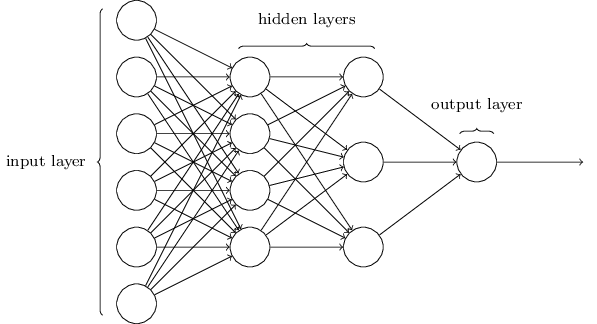
\includegraphics[width=15cm]{utils/tikz11.png}
	\captionof{figure}{Struktura sieci MLP}
	\label{netstructure}
\end{center}

\subsection{Sztuczny neuron}
Pojedynczy neuron pokazany jest na rys. \ref{neuron}. Wykonuje on iloczyn skalarny wektor�w tworzonych przez warto�ci wej�� $x_j$ i odpowiadaj�ce im wagi $w_j$ po czym dodaje do niego wielko�� \textit{bias}:

\begin{equation}
\sum w_jx_j + bias
\end{equation}

Tak otrzymana warto�� jest podawana jako argument funkcji wzbudzenia neuronu. Dopiero wynik tej funkcji jest wynikiem ko�cowym neuronu, \textit{output} na rys. \ref{neuron}.
\newline
\begin{center}
	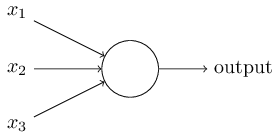
\includegraphics[width=9cm]{utils/neuron.png}
	\captionof{figure}{Pojedy�czy neuron}
	\label{neuron}
\end{center}

\subsection{Funkcja wzbudzenia neuron�w}
Zastosowana funkcja wzbudzenia naszej sieci MLP b�dzie mia�a posta� funkcji sigmoidalnej, przedstawionej na rys. \ref{sigm}.
Funkcja tej postaci zapewnia nam dwie korzy�ci:

\begin{enumerate}
	
	\item Ma�e zmiany wej�� neuron�w b�d� skutkowa�y niewielkimi zmianami na wyj�ciu funkcji sigmoidalnej; pozwoli to kontrolowa� proces uczenia (w przypadku np. funkcji pobudzenia postaci funkcji skokowej, nawet ma�e zmiany wej�� mog� powodowa� nieprzewidywalne zachowanie ca�ej sieci);
	\item Funkcja ta jest r�niczkowalna, co jest kluczowe w algorytmie uczenia wykorzystuj�cym mechanizm wstecznej propagacji (ang. \textit{backpropagation}).
	
\end{enumerate}
\vspace{1cm}
\begin{center}
	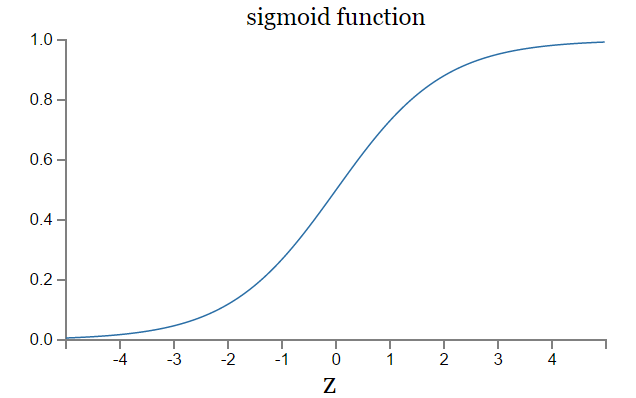
\includegraphics[width=13cm]{utils/sigm.png}
	\captionof{figure}{Posta� funkcji sigmoidalnej}
	\label{sigm}
\end{center}


\subsection{Warstwa wej�ciowa}
Zbi�r MNIST sk�ada si� z 70,000 obrazk�w przedstawiaj�cych pisane r�cznie cyfry. Ka�dy z obrazk�w ma wymiary 28x28, co daje  ilo��  $28*28 = 784$ pikseli na ka�dej ilustracji. Nasza sie� b�dzie posiada�a dok�adnie tyle wej�� - ka�dy z neuron�w warstwy wej�ciowej (\textit{input layer} na rys. \ref{netstructure}) b�dzie otrzymywa� dane z jednego i tego samego dla wszystkich danych pikselu obrazka.

\subsection{Warstwa wyj�ciowa}
Warstwa wyj�ciowa natomiast (\textit{output layer} na rys. \ref{netstructure}) b�dzie sk�ada�a si� z 10 neuron�w: ka�dy z nich b�dzie sygnalizowa� stopie� przynale�no�ci obrazka do danej klasy.

Stopie� przynale�no�ci, jako konsekwencja zastosowania sigmoidalnej funkcji wzbudze� neuron�w, b�dzie zawiera� si� w przedziale $<0, 1>$. Najwi�ksza warto�ci ze zbioru neuron�w wyj�ciowych b�dzie wskazywa�a aktualnie identyfikowan� cyfr�.

\subsection{Proces uczenia}
Do nauki sieci zostanie wykorzystany algorytm wstecznej propagacji (ang. \textit{backpropagation}). Zadanie uczenie sieci przy pomocy tego algorytmu polaga na minimalizacji funckji straty (ang. \textit{loss funtion}) jako funkcji wag i parametr�w bias. Funkcja ta zosta�a przedstawiona jako wz�r  \ref{lossf}, gdzie: $w$ - wagi, $b$ - bias, $n$ - liczebno�� zbioru ucz�cego, $y(x)$ - po��dane wyj�cie dla danego wej�cia,  $a$ - rzeczywisty wynik dzia�ania sieci dla danego wej�cia.

Algorytm ten polega na aplikowaniu do wag drobnych poprawek $\Delta w$ wyliczonych ze wzoru \ref{deltav}, gdzie $ \nabla C$ jest gradientem funkcji strat a $\eta$ jest hiperparametrem wyra�aj�cym wielko�� kroku. 

Skr�towo m�wi�c, po ka�dej iteracji, to jest obliczeniu wyniku dla kolejno wszystkich danych ucz�cych, obliczana jest funkcja $C(w,b)$ i jej gradient, a nast�pnie zmieniane s� wagi w kierunku przeciwnym do  gradientu funcji strat o krok $\eta$.

\begin{eqnarray}  C(w,b) \equiv
\frac{1}{2n} \sum_x \| y(x) - a\|^2.
\label{lossf}
\end{eqnarray}

\begin{eqnarray}
\Delta w = -\eta \nabla C,
\label{deltav}
\end{eqnarray}



\section{Funkcjonalność}

Nasz program będzie na podstawie dostarczonych danych (zbioru MNIST) uczył się rozpoznawać ręcznie pisane cyfry. Proces ten będzie raportowany za pomocą wykresów i statystyk. Gdy sieć zostanie już nauczona, będzie można wprowadzić jako dane wejściowe naszego programu ilustrację, a ten zakomunikuje użytkownikowi, jaka cyfra znajduje się na tym obrazku.
\section{Narz�dzia}

Narz�dzia, z kt�rych zamierzamy korzysta�:

\begin{enumerate}
\item J�zyk programowania: Python	
\item Zewn�trzne biblioteki: Tensorflow
\item �rodowisko programistyczne - JetBrains PyCharm
\item Kontrola wersji - git/GitHub
\item Dokumentacja - narz�dzia LaTeX
\item Komunikacja - Slack
\end{enumerate}
\end{document}
